\chapter{Robótica educativa}

\section{Introducción}

En este capitulo, se tratara de dar cuenta sobre la importancia de la la enseñanza de las ciencias de la computación en la escuela media y como la robótica puede servir de herramienta para lograr ese cometido, aprovechando sus particularidades y ventajas a la hora de abordar conceptos propios del pensamiento algorítmico (repeticiones, recursividad, saltos condicionales, etc.) y tomando como referencia a la actual ley nacional de educación Numero 26.206 que dice: 

\textit{Desarrollar  las  capacidades  necesarias  para  la  comprensión  y  utilización  inteligente  y  crítica  de  los  nuevos  lenguajes  producidos  en  el  campo  de  las tecnologías de la información y la comunicación.}\footnote{art 30 inciso F de la Ley Nro. 26.206 de educación}

Podemos decir que las ciencias de la computación \citep[pág 4]{sadosky2013cc} se volverán de vital importancia a la hora de pensar un esquema curricular especifico para abordar los contenidos básicos propuestos por la ley 26.206.

\section{Antecedentes}

El uso de dispositivos robots para enseñanza, tiene su origen en el trabajo de Seymour Papert, y su desarrollo del lenguaje LOGO. Este lenguaje en un principio accionaba un robot con forma de tortuga (de ahi que el logotipo de LOGO sea una tortuga), el cual se movía sobre una superficie plana dibujando en función de las instrucciones previamente creadas en la computadora que los discentes usaban.

Basado en ese esquema, los discentes programan en lenguaje LOGO (un lenguaje muy parecido en su forma al lenguaje LISP), luego activan el robot tortuga y la computadora enviá las ordenes para que este se mueva, dibujando sobre un papel. A través de esa experiencia, Papert colabora con la empresa LEGO para fabricar el producto LEGO/LOGO, el cual después pasaría a ser conocido como LEGO MINDSTORM\textsuperscript{\texttrademark}, una plataforma física basada en fichas LEGO\textsuperscript{\textregistered} que también incluye hardware de adquisición de datos capas de leer sensores y trabajar sobre diversos actuadores, y permite interconectar todo para lograr diversos robots.

Con el tiempo lenguaje LOGO abandonaría la tortuga robot principalmente por razones presupuestarias, el abaratamiento de las micro computadoras (por ej. COMMODORE\textsuperscript{\textregistered} c64) con capacidad de procesar gráficos a color y el elevado costo de cada robot tortuga, hicieron que fuera muy dificil implementar una curricula basada en LOGO solamente con el uso del robot tortuga.

\subsection{ARDUINO\textsuperscript{\texttrademark} y la revolución del hardware libre.} 

\begin{wrapfigure}{r}{0.5\textwidth}
  \begin{center}
    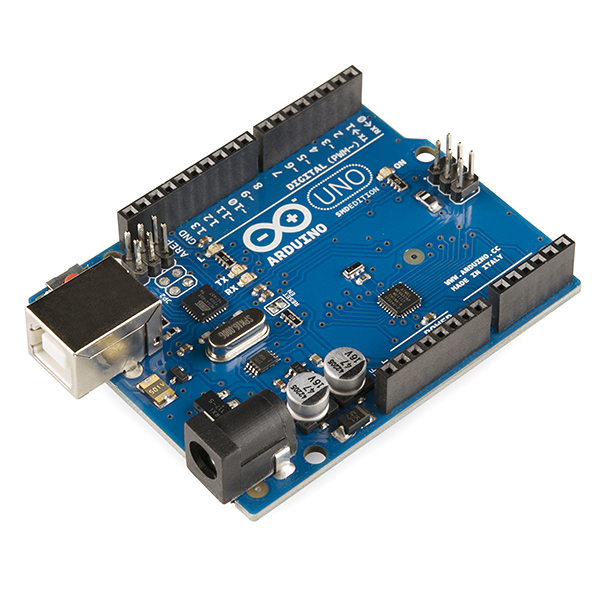
\includegraphics[width=0.4\textwidth]{figuras/Arduino_Uno_-_R3.jpg}
    \caption[Caption for LOF]{Arduino\textsuperscript{\texttrademark} Uno Revisión 3}
       
    \label{fig:arduinouno }
  \end{center}
\end{wrapfigure}

La primera placa Arduino\textsuperscript{\texttrademark} fue introducida en 2005, ofreciendo un bajo costo y facilidad de uso para novatos y profesionales. Buscaba desarrollar proyectos interactivos con su entorno mediante el uso de actuadores y sensores. Su bajo costo y la enorme cantidad de documentación generada por las distintas comunidades de desarrolladores y entusiastas permitió que la plataforma Arduino\textsuperscript{\texttrademark} se volviera un estándar a la hora de hablar sobre automatización o IOT (Internet of things).

Actualmente los miles de kits para enseñanza de robótica que se diseñan y fabrican (a pequeña o gran escala) están basados en la arquitectura Arduino\textsuperscript{\texttrademark} y la serie de micro controladores AVR\textsuperscript{\textregistered} de 8 bits, aprovechando la inmensa documentación y facilidad de adquisición de los componentes, permitiendo también un abaratamiento de costos a causa de la gran demanda que viene suscitándose en los últimos años. Estos kits generalmente constan de una serie uniforme de componentes electrónicos y mecánicos, como servo motores, motores de corriente continua, sensores analógicos / digitales y componentes de electrónica discreta (resistencias, leds, capacitores, etc.), posibilitando trabajar una serie de sistemas de automatización, robótica y/o domotica de mayor o menor complejidad.

%\texttrademark : pone el símbolo TM
%\textregistered : pone el símbolo consistente en una R rodeada de un círculo
%\textcopyright : pone el símbolo consistente en una C rodeada de un círculo
\section{lenguajes de programación en la enseñanza}

En la actualidad y en el marco de la ley nacional de educación 26.206, la enseñanza de la ciencia computacional esta tomando relevancia a nivel de enseñanza, la falta de profesionales especializados en programación y la constante demanda de ''mano de obra'' por parte de la industria del software (software factory) se ha vuelto un factor de preocupación por parte de las autoridades nacionales y distintos planes se están implementando para tratar de paliar esa problemática. Dentro de esos proyectos podemos encontrar el Proyecto \textbf{Escuelas del Futuro}, en la órbita de la Secretaría de Innovación y Calidad Educativa del Ministerio de Educación y Deportes, el cual busca: 

\begin{center}
\textit{
crear un Proyecto con el objeto de generar un cambio transformador en las estrategias pedagógicas y políticas de contenidos para integración del sistema educativo a la cultura digital.
Que para el logro de los objetivos previstos en los considerandos precedentes, resulta conveniente la creación del Proyecto ''Escuelas del Futuro'' orientado a propiciar alfabetización digital de todos/as los/as estudiantes de la Argentina, a través de integración de áreas de conocimiento emergentes, como la programación y la robótica. \footnote{Resolución Ministerial 2.376/16 Ministerio de Educación y Deportes, consultado en http://www.saij.gob.ar/proyecto-escuelas-futuro-nv15957-2016-12-05/123456789-0abc-759-51ti-lpssedadevon?}
} 
\end{center}

Desde esa perspectiva, y como dice la fundación sadosky, la alfabetización digital parte de la enseñanza de las ciencias de la computación pensadas como un conjunto amplio de fundamentos y principios independiente de tecnologías  \citep[pág 12]{sadosky2013cc} que incluyen:

\begin{enumerate}
  \item Programación y algoritmos
  \item Estructuras de datos
  \item Arquitecturas y redes de computadoras
\end{enumerate}

Por otro lado las ciencias de la computación permite fomentar habilidades que pueden ser aplicadas a muchos campos de estudio como:

\begin{enumerate}
  \item Modelización y formalización.
  \item Descomposición en sub problemas.
  \item Generalización y abstracción de casos particulares.
  \item Proceso de diseño, implementación y prueba.
\end{enumerate}

De esta forma la enseñanza de un lenguaje formal toma una particular importancia dentro de el esquema educativo actual, que busca resolver los problemas planteados por la necesidad de alfabetizar digitalmente a la población.

Sin embargo, hay criticas concretas a la enseñanza del ''pensamiento algorritmico'' en contra de una enseñanza de lenguajes formales especificos. La idea de pensamiento algorritmico es que se puede aprender conceptos de programación a través de metas lenguajes, o lenguajes pedagógicos (pseudo código o sistemas basados en diagramas y gráficos). Desde esa perspectiva, un lenguaje educativo permitiría simplificar el contenido técnico complejo, permitiendo abordar de forma escalonada el aprendizaje de la ciencia computacional.

Sin embargo como critica a ese modelo, \cite{dijkstra2010que} plantean que la ''simplificación'' de un lenguaje formal con pseudo codigo o con lenguajes ''de juguete'' (como el caso del lenguaje BASIC en su momento) pueden ser mas  contraproducentes que beneficioso. en dichos del propio dijkstra:

\begin{center}
\textit{It is practically impossible to teach good programming to students that have had a prior exposure to BASIC: as potential programmers they are mentally mutilated beyond hope of regeneration.}
\end{center}

lo que se puede traducir como:

\begin{center}
\textit{Es prácticamente imposible enseñar una buena programación a los estudiantes que han tenido una exposición previa a BASIC: como programadores potenciales son mentalmente mutilados más allá de la esperanza de regeneración.}
\end{center}

seymour \cite{seymour_papert_desafio_1987} plantea que los lenguajes simplificados como BASIC (o como los lenguajes basados en bloques gráficos de mas reciente aparición) que se  ''promocionan'' como lenguajes simples de aprender a causa de su reducido vocabulario, son sin embargo a causa de su escaso vocabulario, extremadamente complejos para poder crear programas que sean algo mas que ''código trivial'', creando lo que seymour \cite{seymour_papert_desafio_1987} llamo el ''fenómeno QWERTY'' por la historia del porque se adopto el tipo de teclado QWERTY en la época de las primeras maquinas de escribir mecánicas (que solían trabarse si se ponían cerca las teclas de uso mas común), pero aun después de la creación de las computadoras (cuando los problemas mecánicos de las maquinas de escribir ya no tenían significado) se siguió usando el teclado QWERTY por costumbre.

\section{Robótica y la enseñanza de programación}

